\begin{figure}[h]
\begin{center}

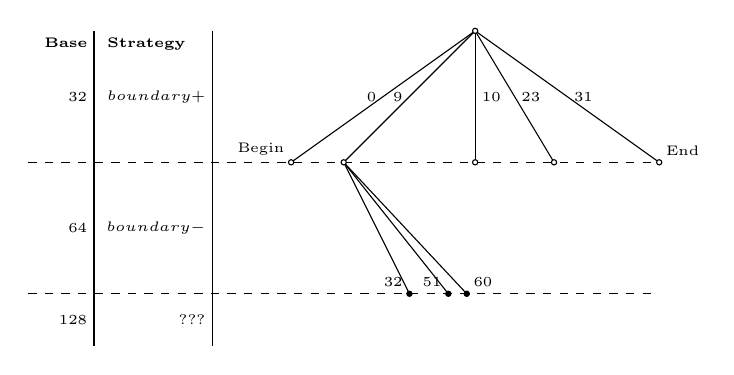
\begin{tikzpicture}[scale=0.95]
\tiny

  \draw (-100pt,0)node[anchor=north east]{\textbf{Strategy}\ \ \ \ }--
        (-100pt,-120pt);
  \draw (-145pt,0)node[anchor=north east]{\textbf{Base}\ }--
        (-145pt,-120pt);
  \draw (-100pt, -25pt) node[anchor=east]{$boundary+$} -- (-100pt, -25pt);
  \draw (-145pt, -25pt) node[anchor=east]{$32$} -- (-145pt, -25pt);
  \draw (-100pt, -75pt) node[anchor=east]{$boundary-$} -- (-100pt, -75pt);
  \draw (-145pt, -75pt) node[anchor=east]{$64$} -- (-145pt, -75pt);
  \draw (-100pt,-110pt) node[anchor=east]{$???$} -- (-100pt,-110pt);
  \draw (-145pt,-110pt) node[anchor=east]{$128$} -- (-145pt,-110pt);
  \draw[dashed] (-170pt,- 50pt) -- (70pt,- 50pt);
  \draw[dashed] (-170pt,-100pt) -- (70pt,-100pt);


  \draw (0,0) -- node[anchor=east]{0}   (-70pt, -50pt);
  \draw (0,0) -- node[anchor=west]{31}  ( 70pt, -50pt);

  \draw (0,0) -- node[anchor=east]{9}  (-50pt, -50pt);
  \draw (0,0) -- node[anchor=west]{10} (  0pt, -50pt);
  \draw (0,0) -- node[anchor=west]{23} ( 30pt, -50pt);

  \draw (-50pt, -50pt) -- (-25.0pt, -100pt);
  \draw (-50pt, -50pt) -- (-10.2pt, -100pt);
  \draw (-50pt, -50pt) -- (- 3.2pt, -100pt);

  \draw[fill=white] (0,0) circle (1pt);

  \draw[fill=white] (-70pt, -50pt) node[anchor=south east]{Begin} circle (1pt);
  \draw[fill=white] ( 70pt, -50pt) node[anchor=south west]{End} circle (1pt);

  \draw[fill=white] (-50pt, -50pt) circle (1pt);
  \draw[fill=white] (  0pt, -50pt) circle (1pt);
  \draw[fill=white] ( 30pt, -50pt) circle (1pt);

  
  \filldraw[black] (-25.0pt, -100pt) node[anchor=south east]{32} circle (1pt);
  \filldraw[black] (-10.2pt, -100pt) node[anchor=south east]{51} circle (1pt);
  \filldraw[black] (- 3.2pt, -100pt) node[anchor=south west]{60} circle (1pt);

\end{tikzpicture}
\caption{Underlying tree model of \NAME{} containing three identifiers at
  depth-1. The randomness makes the first and second element very close regard
  of identifiers ($[9]$ and $[10]$). The sequence requests three other elements
  between these two. The chosen strategy is \emph{boundary--} and since \NAME{}
  doubles the base at each depth, it allocates the fresh identifiers closer of
  $[10.64]$.}
\label{fig:lseqtreeexample}
\end{center}
\end{figure}
